\documentclass[14pt]{extbook}
\usepackage{multicol, enumerate, enumitem, hyperref, color, soul, setspace, parskip, fancyhdr} %General Packages
\usepackage{amssymb, amsthm, amsmath, bbm, latexsym, units, mathtools} %Math Packages
\everymath{\displaystyle} %All math in Display Style
% Packages with additional options
\usepackage[headsep=0.5cm,headheight=12pt, left=1 in,right= 1 in,top= 1 in,bottom= 1 in]{geometry}
\usepackage[usenames,dvipsnames]{xcolor}
\usepackage{dashrule}  % Package to use the command below to create lines between items
\newcommand{\litem}[1]{\item#1\hspace*{-1cm}\rule{\textwidth}{0.4pt}}
\pagestyle{fancy}
\lhead{Progress Quiz 1}
\chead{}
\rhead{Version B}
\lfoot{1269-8776}
\cfoot{}
\rfoot{Fall 2020}
\begin{document}

\begin{enumerate}
\litem{
Write the equation of the line in the graph below in Standard form $Ax+By=C$. Then, choose the intervals that contain $A, B, \text{ and } C$.
\begin{center}
    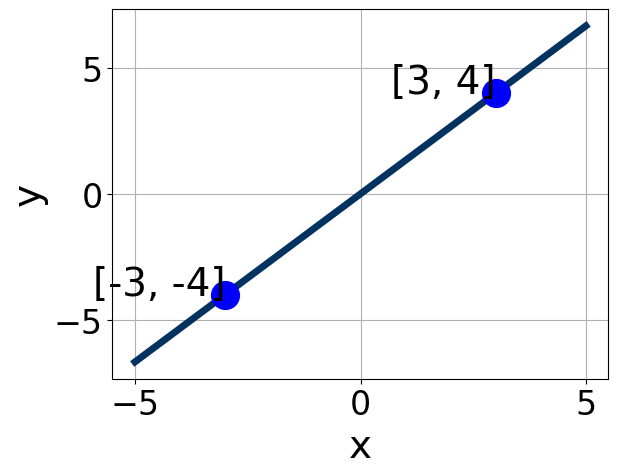
\includegraphics[width=0.5\textwidth]{../Figures/linearGraphToStandardB.png}
\end{center}
\begin{enumerate}[label=\Alph*.]
\item \( A \in [5, 6], \hspace{3mm} B \in [-2.93, -1.4], \text{ and } \hspace{3mm} C \in [-17, -8] \)
\item \( A \in [-6, -1], \hspace{3mm} B \in [-2.93, -1.4], \text{ and } \hspace{3mm} C \in [-17, -8] \)
\item \( A \in [5, 6], \hspace{3mm} B \in [1.71, 2.33], \text{ and } \hspace{3mm} C \in [10, 14] \)
\item \( A \in [-1.5, 3.5], \hspace{3mm} B \in [0.77, 1.64], \text{ and } \hspace{3mm} C \in [2, 6] \)
\item \( A \in [-1.5, 3.5], \hspace{3mm} B \in [-1.8, -0.31], \text{ and } \hspace{3mm} C \in [-8, -2] \)

\end{enumerate} }
\litem{
\begin{enumerate}[label=\Alph*.]

\end{enumerate} }
\litem{
Find the equation of the line described below. Write the linear equation as $ y=mx+b $ and choose the intervals that contain $m$ and $b$.\[ \text{Perpendicular to } 6 x - 7 y = 7 \text{ and passing through the point } (-9, -7). \]\begin{enumerate}[label=\Alph*.]
\item \( m \in [-1.27, -1.11] \hspace*{3mm} b \in [17, 18.1] \)
\item \( m \in [-1.06, -0.59] \hspace*{3mm} b \in [-19.3, -17.3] \)
\item \( m \in [-1.27, -1.11] \hspace*{3mm} b \in [-0.7, 2.6] \)
\item \( m \in [-1.27, -1.11] \hspace*{3mm} b \in [-19.3, -17.3] \)
\item \( m \in [0.97, 1.63] \hspace*{3mm} b \in [2.1, 3.7] \)

\end{enumerate} }
\litem{
First, find the equation of the line containing the two points below. Then, write the equation as $ y=mx+b $ and choose the intervals that contain $m$ and $b$.\[ (-11, -4) \text{ and } (5, 3) \]\begin{enumerate}[label=\Alph*.]
\item \( m \in [-0.09, 0.96] \hspace*{3mm} b \in [-2.94, -1.61] \)
\item \( m \in [-0.09, 0.96] \hspace*{3mm} b \in [-1.26, -0.33] \)
\item \( m \in [-0.09, 0.96] \hspace*{3mm} b \in [6.06, 7.56] \)
\item \( m \in [-0.09, 0.96] \hspace*{3mm} b \in [0.39, 1.44] \)
\item \( m \in [-1.75, -0.21] \hspace*{3mm} b \in [3.58, 6.79] \)

\end{enumerate} }
\litem{
\begin{enumerate}[label=\Alph*.]

\end{enumerate} }
\litem{
Solve the equation below. Then, choose the interval that contains the solution.\[ -3(-18x + 2) = -13(-14x -16) \]\begin{enumerate}[label=\Alph*.]
\item \( x \in [1.47, 1.64] \)
\item \( x \in [1.3, 1.46] \)
\item \( x \in [-0.99, -0.61] \)
\item \( x \in [0.69, 1.06] \)
\item \( \text{There are no real solutions.} \)

\end{enumerate} }
\litem{
Solve the linear equation below. Then, choose the interval that contains the solution.\[ \frac{7x + 3}{3} - \frac{3x -6}{2} = \frac{7x -9}{4} \]\begin{enumerate}[label=\Alph*.]
\item \( x \in [17.64, 22.64] \)
\item \( x \in [4.82, 9.82] \)
\item \( x \in [-0.73, 1.27] \)
\item \( x \in [1.08, 4.08] \)
\item \( \text{There are no real solutions.} \)

\end{enumerate} }
\end{enumerate}

\end{document}